\documentclass[12pt,a4paper]{report}
\usepackage[italian]{babel}
\usepackage{newlfont}
\usepackage{color}
\textwidth=450pt\oddsidemargin=0pt

\usepackage[utf8x]{inputenc}
\usepackage{graphicx}
\usepackage{amsmath}
\usepackage{amssymb}
\usepackage{setspace}

\begin{document}

% qui comincia il titolo
\begin{titlepage}
\begin{center}
{\Large{\textsc{Università degli studi di Roma $\cdot$ Tor Vergata}}}
\rule[0.1cm]{15.8cm}{0.1mm}
\rule[0.5cm]{15.8cm}{0.6mm}
\\\vspace{3mm}

{\small{\bf Macroarea di Lettere e Filosofia \\ Master in Sonic Arts}}

\end{center}

\vspace{23mm}

\begin{center}
\begin{spacing}{1.7}
\textcolor{black}{
\linespread{5}
{\LARGE{\bf
Adattamento del formato ad oggetti Multi-Dimensional Audio MDA alle configurazioni 2.0, 5.1 e 4.0 attraverso la tecnica Vector-Base Amplitude Panning VBAP.
}}}

\end{spacing}
\end{center}

\vspace{50mm} \par \noindent

\begin{minipage}[t]{0.47\textwidth}

{\large{\bf Relatore: \vspace{2mm}\\\textcolor{black}{
Prof. Giuseppe Silvi}\\\\

}
}
\end{minipage}
%
\hfill
%
\begin{minipage}[t]{0.47\textwidth}\raggedleft \textcolor{black}{
{\large{\bf Presentata da:
\vspace{2mm}\\
Lorenzo Ferri}}}
\end{minipage}

\vspace{5mm}

\begin{center}

{\large{%\bf Sessione \textcolor{black}{ I }
%\vspace{2mm}\\

Anno Accademico \textcolor{black}{2016/17}}}
\end{center}

\newpage\null\thispagestyle{empty}

\end{titlepage}
% qui finisce il titolo

\tableofcontents

\listoffigures


\addcontentsline{toc}{chapter}{Elenco delle figure}

\chapter*{Abstract}

L'obbiettivo di questa tesi è quello di implementare un algoritmo che permetta di riprodurre un contenuto sonoro orientato agli oggetti su una configurazione di riproduzione facilmente riscontrabile in un ambiente domestico.

In un primo momento, infatti, andrò a spiegare che cosa sono le \textbf{configurazioni multicanale $\bold{2.0, 4.0}$ e $\bold{5.1}$} ed introdurrò l'audio object-oriented con particolare riguardo al formato ad oggetti \textbf{Multi-Dimensional Audio MDA}.

In un secondo momento cercherò di implementare l'MDA nelle configurazioni multicanale descritte servendomi della tecnica di spazializzazione \textbf{Vector-Base Amplitude Panning VBAP} di cui spiegherò anche il funzionamento.

Infine farò degli esempi.

\addcontentsline{toc}{chapter}{Abstract}

\chapter{Dai canali audio agli oggetti sonori}

Premetto che in questo testo non affronterò tutti gli aspetti della produzione sonora e dell'ascolto, toccherò invece solo quegli aspetti che riguardano la collocazione spaziale degli oggetti sonori\footnote{Con oggetto sonoro intendo quell'entità che contiene l'informazione sonora registrata da un microfono o creata virtualmente che viene elaborata singolarmente in fase di produzione} trattando, quindi, le configurazioni spaziali dei diffusori in fase di produzione in studio e di ascolto a casa.

Nel mondo odierno l'avanzamento tecnologico ha permesso a tutti coloro che ne hanno voglia la possibilità di poter ascoltare un contenuto sonoro in ambiente domestico in modo semplice, basti pensare a chi ascolta un disco musicale in un impianto hi-fi o a chi invece gode dell'ascolto surround\footnote{Con surround si intende quel tipo di ascolto in cui l'ascoltatore è immerso nella scena sonora, per fare questo tipicamente si collocano diffusori ai lati e/o dietro l'ascoltatore} di un film in un impianto home-theater, in tutti questi casi la persona interessata possiede un prodotto sonoro che viene ascoltato attraverso l'impianto audio posseduto in casa, questo è possibile grazie ad una complessa catena di produzione e di ascolto sonoro che da la possibilità a tutti di poter ascoltare il contenuto esattamente come è stato creato.

Quello che sta alla base di tutta questa catena è il produttore, esso per riuscire a creare al meglio il contenuto e per dare la giusta collocazione spaziale agli oggetti sonori deve essere a conoscenza del modo in cui l'ascoltatore ascolta il suo prodotto, infatti esso adotterà un metodo di lavoro che prevede l'allestimento di un impianto audio in studio con le stesse specifiche spaziali (posizione e numero di diffusori) di quello che normalmente adotterebbe l'ascoltatore in casa, scegliendo questa soluzione è sicuro di creare un prodotto con la giusta collocazione spaziale di ogni oggetto sonoro e che l'ascoltatore senta la medesima cosa.

Successivamente, il produttore riverserà il contenuto sonoro codificato in certo formato\footnote{Con formato audio intendo il protocollo e le specifiche con cui è creato e memorizzato un contenuto sonoro all'interno di un supporto} all'interno di un supporto che verrà poi acquistato dall'ascoltatore e riprodotto in casa dal suo impianto, logicamente l'impianto deve avere un lettore in grado di poter supportare il formato e in grado (attraverso specifiche decodifiche) di associare a ogni diffusore un canale audio da riprodurre.

Per fare un esempio, consideriamo l'ascolto di un disco in un impianto hi-fi, nella maggior parte dei casi in cui della musica sia creata in studio di registrazione si opera in modo che per tutta la sua produzione si rispetti un certo standard nella collocazione dei monitor all'interno dello studio, stessa cosa dovrebbe fare l'ascoltatore a casa per usufruire della stessa informazione musicale, infatti in questo caso sia i fonici che l'ascoltatore dovrebbero rispettare lo standard dato dalla configurazione 2.0 contenuta nella specifica \cite{5.1} per rientrare nel modo più comune di produzione ed ascolto di contenuti puramente musicali.

Stesso discorso si può fare per l'ascolto surround di contenuti sonori di un film solo che in questo caso, sia in studio che a casa, si a avrà una configurazione adatta rispettivamente alla creazione e alla riproduzione di un suono surround tipico di una pellicola cinematografica, una configurazione possibile e che è la maggiore impiegata in ambito domestico è la 5.1 data anch'essa dalla specifica \cite{5.1}.

In tutti due i casi il produttore e l'ascoltatore seguono lo stesso standard di collocazione spaziale dei diffusori , quindi di conseguenza quest'ultimo ascolterà esattamente quello che il produttore vuole che si senta (si parlerà sempre di collocazione degli oggetti sonori); spesso però capita che l'ascoltatore non è in possesso un impianto in grado di riprodurre spazialmente il contenuto di un prodotto sonoro (per esempio basti pensare a chi vuole sentire un audio surround di un film in un comune hi-fi) e che quindi non in grado di rispettare lo standard della catena sopra proposta.

In questi casi esistono degli algoritmi che a patto di sacrificare la corretta ricostruzione dell'ambiente sonoro, riescono a far riprodurre in un impianto configurato spazialmente in una certa maniera un prodotto musicale non destinato nativamente ad esso.

Ora, prima di trattare un esempio di uno di questi algoritmi, è d'obbligo fermarsi un attimo e percorrere brevemente quali sono le specifiche degli standard appena citati e introdurre la configurazione $4.0$ che tratterò in questa tesi.

\section{Configurazioni di riproduzione 2.0, 5.1 e 4.0}\label{metodi}

Nell'audio, quando si parla di configurazione spaziale, è norma usare un codice numerico standard che sta ad indicare sinteticamente il numero di diffusori sonori usati e la loro funzione, questo codice è composto da tre numeri separati da punti nel formato $X.Y.Z$ dove $X$ sta ad indicare il numero di diffusori disposti orizzontalmente sul piano attorno l'ascoltatore, $Y$ sta ad indicare il numero di diffusori imputati alla riproduzione del canale LFE\footnote{LFE (acronimo di Low Frequency Effect) è quel canale imputato alla riproduzione degli effetti a bassa frequenza tipicamente riprodotti da uno o più subwoofer} e $Z$ sta per il numero di diffusori posti sopra l'ascoltatore per ampliare l'ascolto anche verticalmente.

La prima configurazione descritta è la \textbf{2.0} che come da specifica ITU-R BS.775-3\cite{5.1} prevede l'utilizzo di due diffusori (di norma full-range\footnote{In realtà si potrebbe usare anche un subwoofer in aiuto ai due diffusori per quanto riguarda la zona frequenziale bassa (tipicamente sotto i 120 Hz}) posti di fronte all'ascoltatore con angoli di $\pm 30°$ rispetto la linea mediana perpendicolare alla testa dell'ascoltatore come in figura \ref{fig:2.0}.

Tipicamente la sensazione di collocazione spaziale di una sorgente sonora in questa configurazione viene data dalla differenza di potenza del segnale inviato ai due diffusori, infatti se il segnale risulta più forte in uno dei due, la sorgente fantasma risulterà più spostata verso quest'ultimo in accordo con la tangent law scritta in \cite{vbap}.

E' consuetudine indicare con L (left) ed R (right) il diffusore posto rispettivamente di fronte a sinistra e a destra dell'ascoltatore.

\begin{figure}[htbp]
	\centering
	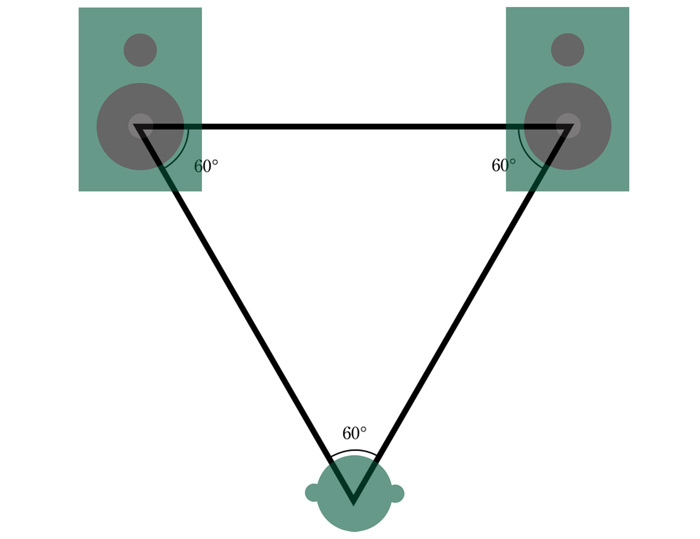
\includegraphics[scale=0.50]{figures/2-0.jpg}
	\caption {Configurazione 2.0 (ITU-R BS.775-3)}
	\label{fig:2.0}
	\end{figure}
	
Per quanto riguarda un ascolto surround, invece, diverse sono le configurazioni possibili ma quella che interessa a noi è la 5.1 data dalla specifica ITU-R BS 775-3\cite{5.1}.

Questa configurazione spaziale (quasi sicuramente la più diffusa in ambito surround domestico) è composta da 5 canali distribuiti in 5 diffusori disposti rispettivamente a $0°$, $\pm30°$ e $\pm110/120°$ e un canale LFE riprodotto da un subwoofer posto tipicamente davanti l'ascoltatore (In realtà il collocamento del subwoofer non è strettamente indicato nelle specifiche in quanto la natura delle basse frequenze le rende omnidirezionali, invece nelle specifiche è riportato il fatto che il canale LFE deve avere un incremento del segnale di $+10dB$.

In figura \ref{fig:5.1} possiamo vedere come sono disposti i 5 diffusori ma è da notare che non è riportata la posizione del subwoofer per il discorso appena affrontato.

E' norma indicare i diffusori come C (center) per il diffusore centrale, L (left) ed R (right) per i diffusori rispettivamente a $\pm30°$ (è consuetudine poi usare casse full-range per la coppia L-R), LS (left-surround) ed RS (right-surround) per i diffusori rispettivamente a $\pm110/120°$ .

\begin{figure}[htbp]
	\centering
	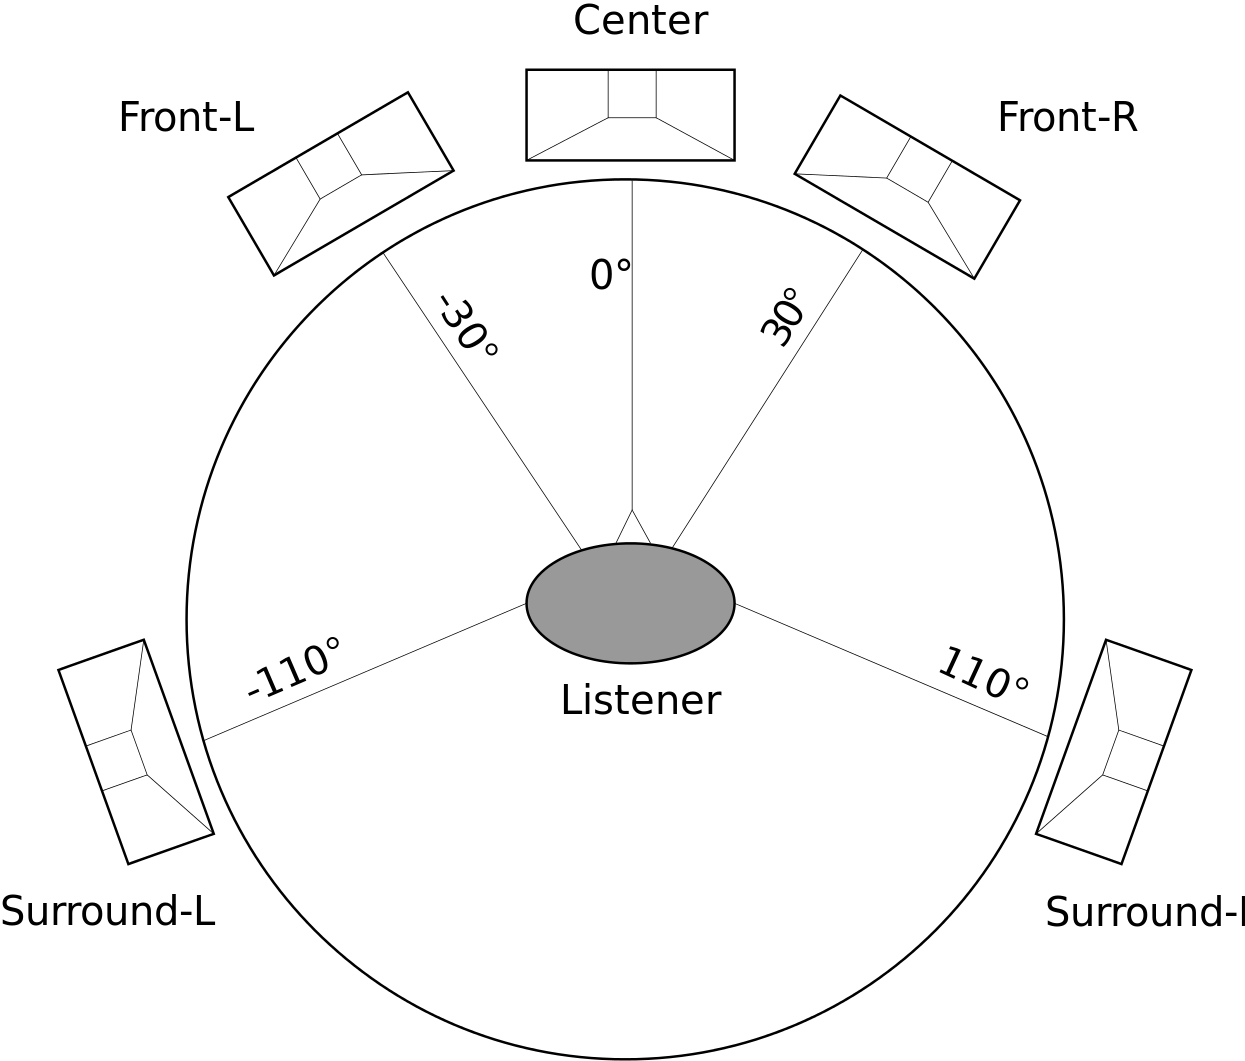
\includegraphics[scale=0.18]{figures/5-1.png}
	\caption {Configurazione 5.1 (ITU-R BS.775-3)}
	\label{fig:5.1}
	\end{figure}

In parallelo una configurazione utilizzata in passato che si potrebbe trovare in ambito domestico è la 4.0; questa tecnica prevede l'utilizzo di 4 diffusori posti sui vertici di un quadrato, cioè con angoli di $\pm45°$ e $\pm135°$ con al centro l'ascoltatore.

Usualmente in letteratura si denominano la coppia di diffusori posti di fronte come LF (left-front) - RF (right-front) e la coppia posta dietro come LB (left-back) - RB (right-back), questi per riprodurre al meglio il contenuto sonoro dovrebbero essere full-range.

Per quanto riguarda questa configurazione (si veda \cite{surround}) c'è da dire che questa disposizione crea dei problemi di percezione del contenuto spaziale in quanto il nostro udito è più sensibile a ciò che proviene di fronte a noi (si veda figura \ref{fig:quadrifonia}), questo costituisce un problema per i nostri scopi ma prenderemo lo stesso la configurazione in considerazione in quanto è possibile che in ambito domestico qualcuno possieda ancora un impianto 4.0.

\begin{figure}[htbp]
	\centering
	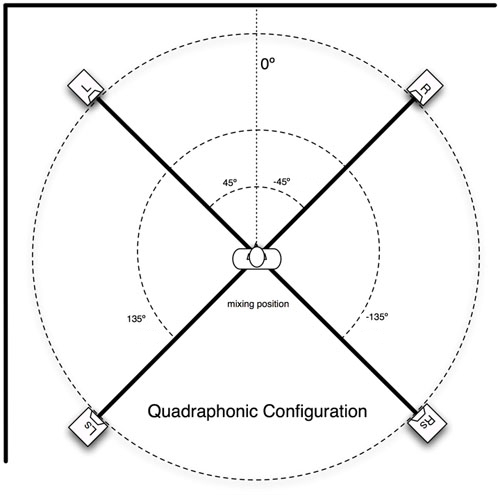
\includegraphics[scale=0.40]{figures/quad.jpg} 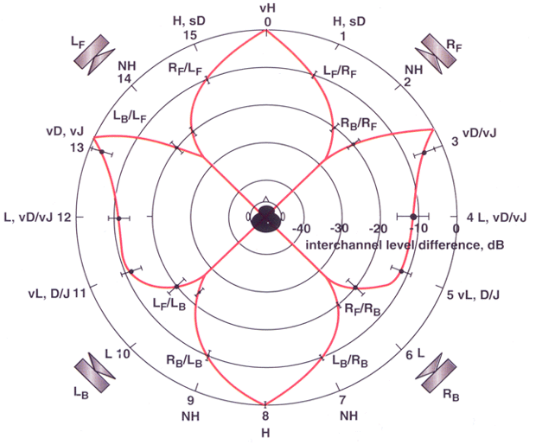
\includegraphics[scale=0.45]{figures/farfalla.png}
	\caption {Configurazione 4.0 e relativa percezione spaziale}
	\label{fig:quadrifonia}
	\end{figure}

\[\thicksim\blacklozenge \thicksim \]

Abbiamo visto quindi che lo stesso standard sulla collocazione spaziale dei diffusori dovrebbe essere mantenuta dalla fase di produzione a quella di ascolto per avere un ascolto ottimale, ma prima ho accennato del fatto che non è sempre così, infatti è possibile ascoltare in un impianto configurato secondo una certa specifica un contenuto sonoro non creato per esso con l'ausilio di algoritmi che permettono di rendere le configurazioni spaziali dei diffusori intercambiabili.

Per fare un esempio, la specifica ITU-R BS.775-3 definisce il modo in cui posso adattare un prodotto sonoro in una configurazione 2.0 ma che originariamente è stato creato per un 5.1.

L'algoritmo si basa su una decodifica matriciale, quest'ultima la ottengo combinando linearmente i canali della configurazione di partenza per ottenere quelli di arrivo, infatti nel testo è presente una matrice dove in ingresso abbiamo 5 dei canali del 5.1 ed in uscita abbiamo i 2 canali del 2.0, risulta che L' ed R' sono combinazione lineare di L, R, C, LS, RB secondo i coefficienti tabulati sotto.

\begin{figure}[htbp]
	\centering
	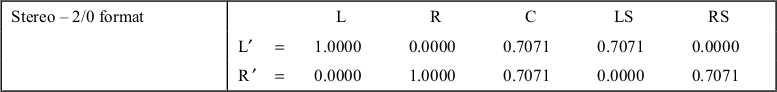
\includegraphics[scale=0.5]{figures/5-1to2-0.png}
	\caption {Matrice di decodifica da 5.1 a 2.0}
	\label{fig:decodifica}
	\end{figure}

Per quanto riguarda il canale LFE esso va aumentato di $+10dB$ prima di ripartirlo nei due canali L ed R (ad ogni ripartizione poi va scalato di $-6dB$ per controbilanciare il raddoppio del segnale).

Abbiamo visto quindi un esempio di algoritmo che rende un contenuto sonoro adatto ad una riproduzione 5.1 intercambiabile con un 2.0.

\section{Formato audio object-oriented}

Ora capito quali sono i principali standard di riproduzione ci interessa capire il legame che c'è tra formato audio, canale audio e riproduzione in un impianto. 

Abbiamo detto in precedenza che il produttore riversa in un supporto il contenuto sonoro in certo formato, non ci interessano tanto le specifiche che stanno alla base di quest'ultimo ma ci interessa capire che ogni formato prevede al suo interno l'esistenza di un certo numero flussi di segnale, questi ultimi andranno a costituire, con o senza opportune codifiche, i canali audio per poter pilotare l'impianto, faccio un esempio.

Il formato Dolby Digital 5.1 (si veda \cite{digital}) prevede al suo interno 6 flussi di segnale indipendenti dove ognuno andrà a costituire un canale audio differente, invece il formato Dolby Surround (si veda \cite{surround}) prevede al suo interno 2 flussi di segnale che con un opportuna codifica (sistema matriciale) andranno a costituire i 4 canali audio per pilotare l'impianto. 

\begin{figure}[htbp]
	\centering
	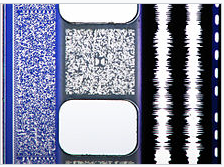
\includegraphics[scale=0.5]{figures/pellicola.png} \ \ \ \ \ \ \ \ \ \ \ \ \ \ \ \ 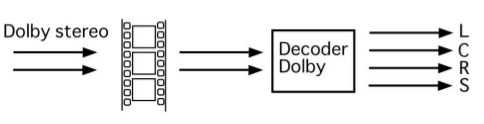
\includegraphics[scale=0.5]{figures/dolbysurround.png}
	\caption {Pellicola in dolby digital 5.1 e catena del segnale di dolby surround}
	\label{fig:pellicola}
	\end{figure}

Detto questo non è difficile capire il fatto che i flussi di segnale all'interno di un formato sono in stretto contatto con i canali audio e con la configurazione spaziale in quanto possiamo pensare, in un certo senso, che i flussi contengono l'informazione da far riprodurre all'impianto, quindi il produttore deve sapere già dalla fase iniziale cosa far riprodurre a quale diffusore, cosa che non non avviene nell'\textbf{audio orientato agli oggetti}.

Da un po di tempo l'avanzamento tecnologico nel campo dell'intrattenimento del grande schermo ha cercato di soddisfare una tendenza a creare un audio avvolgente e ad effetto all'interno delle sale, cominciando con l'introduzione dell'audio surround fino ad arrivare ai giorni nostri a introdurre oggetti sonori in movimento all'interno del cinema di cui l'ascoltatore può distintamente riconoscere la provenienza.

Per esempio la Dolby laboratories ha già implementato una tecnologia in grado di fare questo, nel suo ultimo brevetto \textbf{Dolby Atmos} (si veda documentazione \cite{atmos}) ha implementato nel formato di riproduzione anche una parte dedicata agli oggetti sonori, infatti oltre ad avere un tappeto sonoro dato dalla configurazione 7.1, il formato di dolby atmos permette la memorizzazione di 128 oggetti indipendenti collocati nello spazio sonoro 3D tramite coordinate spaziali, sarà poi il DSP a valle che in questo farà parte della catena Dolby Atmos che, conoscendo le coordinate di ogni oggetto, farà riprodurre ai diffusori il giusto segnale per far si che l'ascoltatore senta l'oggetto sonoro proveniente da un punto preciso.

Logicamente anche in questa catena qualcuno o qualcosa dovrà conoscere la disposizione dei diffusori ed è qui la differenza fondamentale, nell'audio standard è il produttore che crea il contenuto a conoscere la configurazione dell'impianto in cui verrà riprodotto quindi sarà vincolato ad esso, invece nell'audio ad oggetti il produttore è molto più slegato dalla configurazione spaziale in quanto nei formati object-oriented non c'è nessun riferimento a quale diffusore andrà riprodurre cosa, sarà poi il DSP dell'impianto di riproduzione ad occuparsi di questo compito.

Per il discorso appena fatto si veda l'articolo \cite{object}.

Questo sostanzialmente sta alla base dell'audio ad oggetti, nel prossimo capitolo vedremo come implementare concretamente questo procedimento.

\chapter{Formato MDA e Spazializzatore 3D} \label{dolby}

L'idea per la realizzazione pratica dell'audio ad oggetti comincia in fase di produzione, bisogna scordarsi della fase di downmix\footnote{Con downmix intendo quel procedimento all'interno della catena produttiva musicale in cui passo dalla totalità dei canali formanti un progetto ai canali previsti nel formato di riproduzione} e scordarsi del panner installato in banchi mixer o in software DAW classici intraprendendo una strada diversa, vediamo i passaggi:

 \begin{enumerate}
 
\item Si devono preparare e disporre degli oggetti sonori esattamente con l'informazione sonora voluta, questo passaggio non sarebbe altro che il risultato della pre-produzione di ogni oggetto.
\item Si crea attraverso un software apposito (sotto forma di stand-alone o di plug-in) uno spazio di riproduzione virtuale e si dispongono questi oggetti in esso attraverso delle coordinate spaziali (chiamerò questo software panner 3D).
\item Le informazioni sonore di ogni oggetto e le relative coordinate spaziali verranno memorizzate nel supporto attraverso un opportuno format a oggetti standardizzato adatto al nostro scopo (in realtà oltre che alla posizione il format terrà conto anche di altri parametri come grandezza, volume ecc...).
 \end{enumerate}

Parlando fino ad ora di Dolby è plausibile che analizzeremo come formato e come software di spazializzazione 3D quello proprietario di Dolby Atmos ma il fatto è che, essendo questa tecnologia soggetta a brevetto, essa é chiusa a sole applicazioni che riguardano il mondo Dolby, altri marchi hanno cercato di produrre formati proprietari simili ma sempre vincolati da brevetto, marchi quali Auro3D per citarne uno, ma noi ricerchiamo qualcosa che sia un formato open in grado di adattarsi e a diventare uno standard. 

\section{Formato MDA}

Si veda \cite{mda} per la documentazione riguardante questo paragrafo.

L'azienda californiana \textbf{Digital Theater System DTS} (storica rivale di Dolby per quanto riguarda le tecnologie di riproduzione di audio per film) anche lei interessata all'audio ad oggetti ha creato un formato libero che fa esattamente al caso nostro, questo formato prende il nome di Multi-Dimensional Audio, o abbreviato, MDA.

Questo si compone al suo interno di una parte dedicata alla riproduzione multicanale classica che permette la creazione di un tappeto sonoro in una configurazione surround voluta e di una parte dedicata agli oggetti sonori nella quale contenere le informazioni necessarie alla loro successiva riproduzione, infatti possiamo trovare memorizzati all'interno del formato una serie di segnali costituenti gli oggetti sonori e dei \textbf{metadati} in cui sono incapsulati dei parametri necessari al loro corretto posizionamento spaziale.

Principalmente i parametri contenuti nei metadati sono:

\begin{itemize}\label{aaa}
\item \textbf{Position}: sono un set di 3 valori che indicano la posizione dell'oggetto sonoro in relazione con la posizione dell'ascoltatore che avrà come valori la terna (0,0,0).

Considerando lo spazio virtuale costruito sull'asse $X$ posto di fronte all'ascoltatore, l'asse $Y$ posto di fianco e l'asse $Z$ posto verso l'alto come in figura \ref{fig:coordinate}, nei metadati sono inseriti i valori relativi all'angolo di azimut $\theta$, l'angolo di elevazione $\phi$ e il raggio $r$ costituenti le coordinate sferiche.

All'occorrenza una relativa trasformazione a coordinate cartesiane posso farla in questo modo:

\begin{equation}
\left\{\begin{matrix}
\theta = arctg \left(\dfrac{y}{x} \right) \\
\phi   = arctg \left(\dfrac{\sqrt{x^2 + y^2 }}{z} \right) \\
r = \sqrt{x^2 +y^2 +z^2 }\\
\end{matrix}\right.	 \ \ \Rightarrow \ \  \left\{\begin{matrix}
x= r\ cos(\theta) cos(\phi) \\
y= r\ sin(\theta) cos(\phi)\\
z= r\ sin(\phi)\\
\end{matrix}\right.
	\label{eq:coordinatepolari}
\end{equation}

\begin{figure}[htbp]
	\centering
	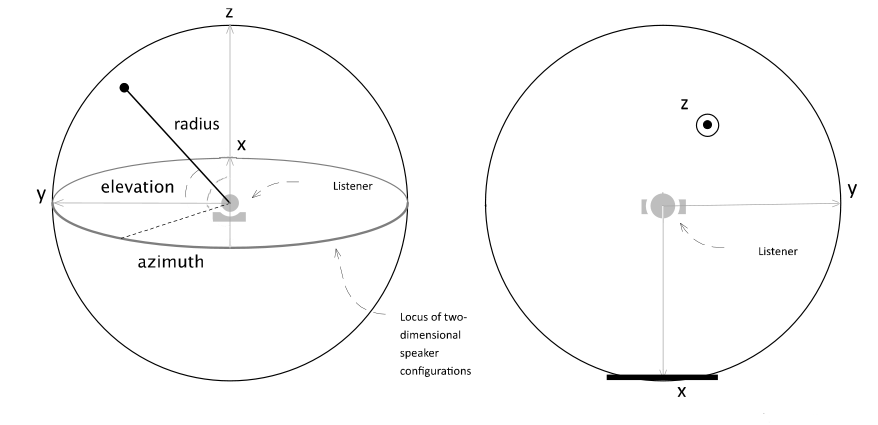
\includegraphics[scale=0.40]{figures/azimut.png}
	\caption {Coordinate spaziali sferiche}
	\label{fig:coordinate}
	\end{figure}

\item \textbf{Uniform Resource Identifier}\cite{uri} definito con la sigla URI é un indirizzo che identifica il bitstream\footnote{Con bitstream si intende le sequenza binaria che contiene un'informazione} dell'oggetto sonoro in maniera univoca (lo stesso URI non può riferirsi a due bitstream).

\item \textbf{ID} è un indirizzo che identifica in modo univoco un object nella timeline (anche qui lo stesso ID non può riferirsi a due oggetti diversi).

\item \textbf{Gain}: è un coefficiente numerico con un range di valori compreso tra $[-411,100]/4 \ dB$, esso  collegato alla quantità di segnale dell'oggetto riprodotto in quanto tramite la trasformazione data dalla formula \ref{db} possiamo vedere come viene scalato o incrementato il segnale dell'oggetto per la sua successiva riproduzione.

\begin{equation}
sgn_{post\_gain}(t)= sgn_{pre\_gain}(t) \cdot 10^{\frac{g[dB]}{20}}
\label{db}
\end{equation}

Da notare che si possono riscontrare due valori di gain nei metadati, questo descritto sopra è riferito alla sorgente monofonica che costituisce un singolo oggetto sonoro (monosource-fragment), l'altro invece è riferito all object-fragment che definirò in seguito, quest'ultimo però avendo un range di valori con valore massimo di $0\ dB$ non permette un aumento del segnale complessivo dell'object-fragment.
 
\item \textbf{Aperture}: è un parametro che indicherebbe l'estensione dell'oggetto sonoro da ricreare , ha un range di valori compreso tra $[0,255]*(180/255)\ °$ (più l'oggetto è grande più gli altoparlanti posti marginalmente della sorgente fantasma si attivano, esempio se il valore fosse $225$ allora si attiverebbero tutti i diffusori). 

\item \textbf{Divergence}: anch'esso espresso in gradi quantifica la grandezza che deve avere l'oggetto sonoro ma solo sul piano orizzontale, ha un range di valori di $[0,255]*(180/255)\ °$ dove il valore indica l'estensione in gradi di metà dell'arco costituente l'oggetto esteso, un esempio più esplicativo si ha in figura \ref{fig:apertura}.

	\begin{figure}[htbp]
	\centering
	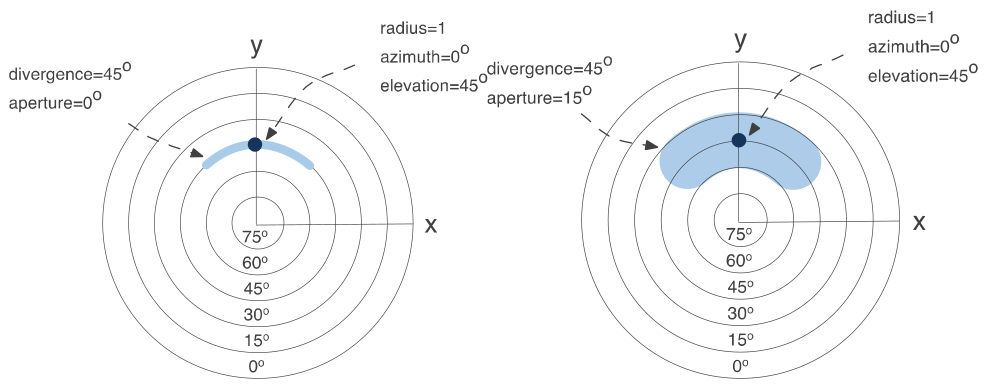
\includegraphics[scale=0.35]{figures/apertura.png}
	\caption {Parametri di apertura e divergenza}
	\label{fig:apertura}
	\end{figure}

\item \textbf{Coherent}: è un valore che può definire la riproduzione in modo coerente (value=0) o incoerente (value=1) dell'oggetto sonoro se quest'ultimo viene esteso a più diffusori tramite i parametri divergence e aperture .

\end{itemize}

Questi sono i principalmente i parametri scritti nei metadati che ci servono per la spazializzazione, bisogna ora affrontare il concetto di object-fragment.

Consideriamo un oggetto sonoro, l'informazione sonora che lo descrive vive nel nel suo bitstream, all'interno del formato la più piccola entità che tiene conto di questo flusso di dati si chiama \textbf{monosource-fragment}, infatti in quest'ultimo è presente un riferimento ai sample attraverso il parametro URI con in aggiunta il gain sopra proposto in modo da caratterizzare staticamente l'oggetto (cioè l'oggetto è caratterizzato solo da informazione che non tengono conto del suo spostamento o variazione).

\begin{figure}[htbp]
	\centering
	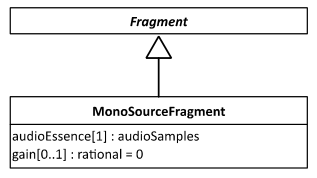
\includegraphics[scale=0.50]{figures/monosource-fragment.png}
	\caption {Monosource-fragment}
	\label{fig:msf}
	\end{figure}

Consideriamo invece lo stesso oggetto che si muove nello spazio, i soli valori del monosource-fragment non bastano a caratterizzare la sua dinamicità, infatti il formato prevede la creazione di una nuova entità di nome \textbf{Object-Fragment} che fa rifermento al monosource-fragment ma che ha in aggiunta il restante dei metadati sopra descritti per rendere l'oggetto posizionabile nel tempo.

Normalmente per far si che ci sia una variazione di provenienza dell'oggetto, all'interno del object-fragment i valori dei metadati sono funzione del tempo della timeline.

\begin{figure}[htbp]
	\centering
	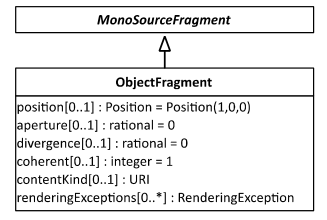
\includegraphics[scale=0.50]{figures/object-fragment.png}
	\caption {Object-fragment}
	\label{fig:of}
	\end{figure}
	 
Appunto per quanto riguarda la parte di sincronizzazione del formato, è posto al di sopra di tutto una timeline (figura \ref{fig:time}) che ha la funzione di richiamare gli object-fragment quando servono, essa è suddivisa in segmenti temporali di durata $\dfrac{1}{f_c}$ dove $f_c$ è la frequenza di campionamento impostata per la totalità degli oggetti sonori\footnote{L'informazione della $f_c$ è contenuta negli header del formato} e dove a ogni segmento è associato una lista contenente gli ID che richiamano gli object-fragment da riprodurre, un esempio esplicativo è dato dallo schema \ref{fig:object}.

\begin{figure}[htbp]
	\centering
	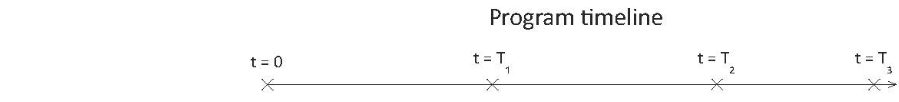
\includegraphics[scale=0.50]{figures/timeline.png}\\
	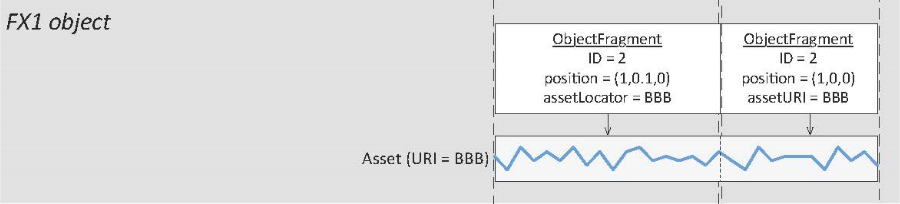
\includegraphics[scale=0.50]{figures/object1.png}\\
	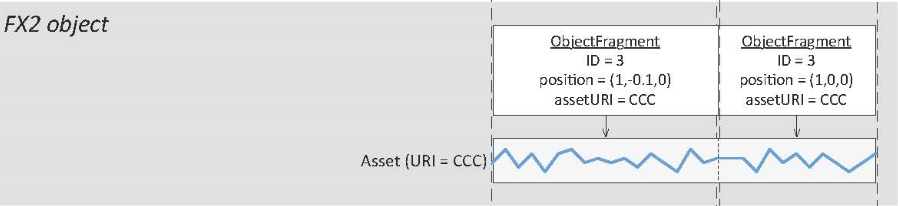
\includegraphics[scale=0.50]{figures/object2.png}\\
	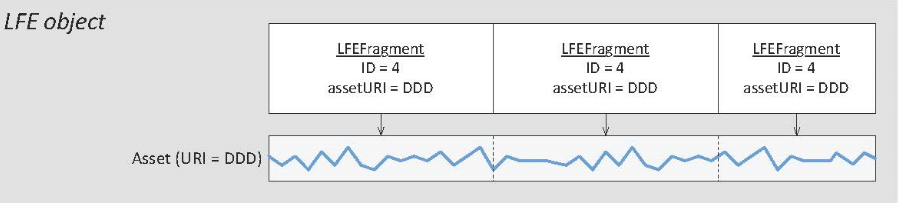
\includegraphics[scale=0.50]{figures/object3.png}
	\caption {Schema esplicativo funzionamento formato MDA}
	\label{fig:object}
	\end{figure}

\begin{figure}[htbp]
	\centering
	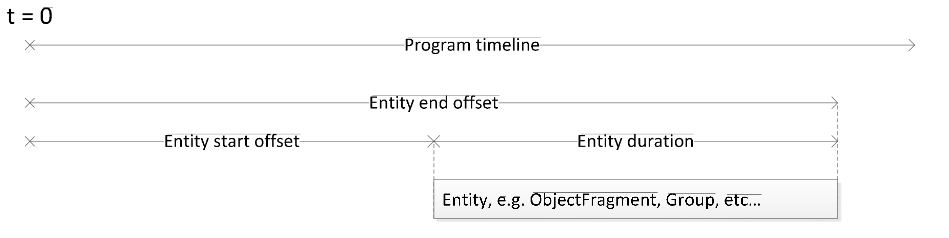
\includegraphics[scale=0.50]{figures/timeline2.png}
	\caption {Azione di richiamo di un object-fragment}
	\label{fig:time}
	\end{figure}

In questo caso, in figura \ref{fig:object}, il lasso di tempo fra $T1$ e $T2$ è caratterizzato dal richiamo degli oggetti con $ID=1,2,3,4$ ognuno di questi caratterizzato da metadati indicanti la posizione e il bitstream da riprodurre tramite l'ID, nel lasso di tempo successivo vediamo che sono in riproduzione gli stessi object-fragment con gli stessi ID ma in questo caso con posizioni diverse il che fanno spostare virtualmente gli oggetti sonori nello spazio virtuale.

Da notare che è presente anche un LFE-Object con $ID=4$ in cui non è segnata la posizione, questo perché data la natura omnidirezionale delle basse frequenze non avrebbe senso collocare spazialmente il monosource-object, e se per assurdo prendessimo questa affermazione come errata non avrebbe comunque utilità indicare la posizione in quanto di solito si avrà un solo subwoofer che, grazie alla sua estensione delle frequenze verso il basso, è in grado di riprodurre un oggetto contenuto nell'LFE.

%da qui devo controllare

\subsection{Formato MDA per riproduzione audio}

Qui faccio una piccola annotazione personale per quanto riguarda l'MDA per soli fini musicali.

Nella maggior parte dei casi quando si fa musica in studio di registrazione è abbastanza difficile che abbiamo oggetti sonori in movimento e di dimensioni che variano nel tempo, quindi si potrebbe fare una piccola modifica al formato che, essendo principalmente stato creato per il cinema, avrà attributi in eccesso che per la sola riproduzione musicale.

Sostanzialmente abbiamo tre tipi di oggetti sonori in un programma puramente musicale: oggetti fermi, oggetti oscillanti tra due punti ed oggetti costituiti da effetti spaziali; tutti questi oggetti possono essere pensati come statici quindi con coordinate ed estensione fissa, in questo caso si potrebbe alleggerire il formato in quanto non avrebbe più senso parlare di metadati che cambiano perché per l'intera esecuzione del brano si avrebbero, all'interno di un object-fragment, solo un set di metadati fissi nel tempo, quindi si possono direttamente assegnare questi metadati fissi all'oggetto sonoro al primo istante di richiamo da parte della  timeline senza ripetere lo stesso set ad ogni $T=\frac{1}{f_c}$.

Per quanto riguarda gli oggetti statici questo trucco calza alla perfezione, per gli effetti che di solito cercano di dare una sensazione di immersione, come potrebbe essere un riverbero per esempio, basterà avere come oggetto il solo contenuto del brano riverberato e assegnarli una giusta divergenza, apertura e coerenza; per quanto riguarda gli oggetti oscillanti (come potrebbe essere un tremolo fatto con un pan-pot in una tastiera) basterà creare in fase di post-produzione due oggetti diversi che hanno lo stesso contenuto sonoro e che differiscono soltanto per il fatto che l'intensità sonora $I'=\alpha \ \ (0\leq \alpha \leq 1)$ di un oggetto corrisponderà a una intensità $I''=(1-\alpha) I$ del secondo oggetto (dove $I$ é l'intensità totale che dovrebbe avere originariamente l'oggetto se fosse riprodotto interamente in un solo punto).

\section{Spazializzatore 3D}

Precedentemente abbiamo visto le specifiche a noi utili del formato MDA, ora non ci rimane introdurre il software di spazializzazione 3D.

Come spiegato, nel workflow di produzione, bisognerà fermarsi prima del down-mix e bisognerà prendere un qualche software di spazializzazione 3D che sia in grado di interfacciarsi con il mondo object-oriented dell'MDA, diverse aziende stanno sviluppando soluzioni di questo tipo in quanto vogliono interfacciarsi a questo formato open ed in qualche modo creare un collegamento tra il loro formato proprietario e l'MDA.

Per esempio la Dolby utilizza un panner 3D per Dolby Atmos che supporta anche il riversamento del contenuto il formato MDA, anche la Auro Technologies ha adottato la stessa politica o in alternativa anche la software-house Fairlight ha creato uno spazializzatore di nome 3DAW (secondo me molto interessante) che supporta anche esso l'MDA.

Detto questo, ricercando uno spazializzatore adatto, la mia attenzione è ricaduta sull'\textbf{MDA creator} proprietario della DTS in quanto è la scelta più intuitiva e la migliore per integrazione in quanto DTS è l'ideatrice sia del panner 3D che del formato.

Tutte le informazioni su MDA creator verranno prese dal suo manuale \cite{creator}.

Questo plugin disponibile solo per Protools è di semplice comprensione, bisogna mettere in insert in ogni traccia questo plugin (condizione necessaria è che tutte le tracce devono avere la stessa lunghezza), poi aprendo l'interfaccia del panner bisognerà posizionare ogni oggetto nel punto in cui si desidera e con divergenza e apertura voluta (si veda il paragrafo \ref{aaa} per sapere i parametri del formato), logicamente questi parametri possono essere automatizzati per spostare e modificare l'oggetto nel tempo.

Inoltre si possono creare dei ''Bed Object'' che sarebbero oggetti i quali potranno essere direttamente codificati nel sistema di riproduzione scelto (esempio classico è la colonna sonora in 5.1 nei film) ai quali verranno sommati gli oggetti veri e propri del formato.

Una volta fatto questo l'MDA creator metterà a disposizione tre scelte di output, quella che interessa a noi è la modalità di esportazione con MDA file: questa scelta ci porta alla creazione dei file \textbf{.map, .mix} e \textbf{.mda} dove quest'ultimo è proprio il file contenente i metadati e gli oggetti sonori proposti in questo formato.

\begin{figure}[htbp]
	\centering
	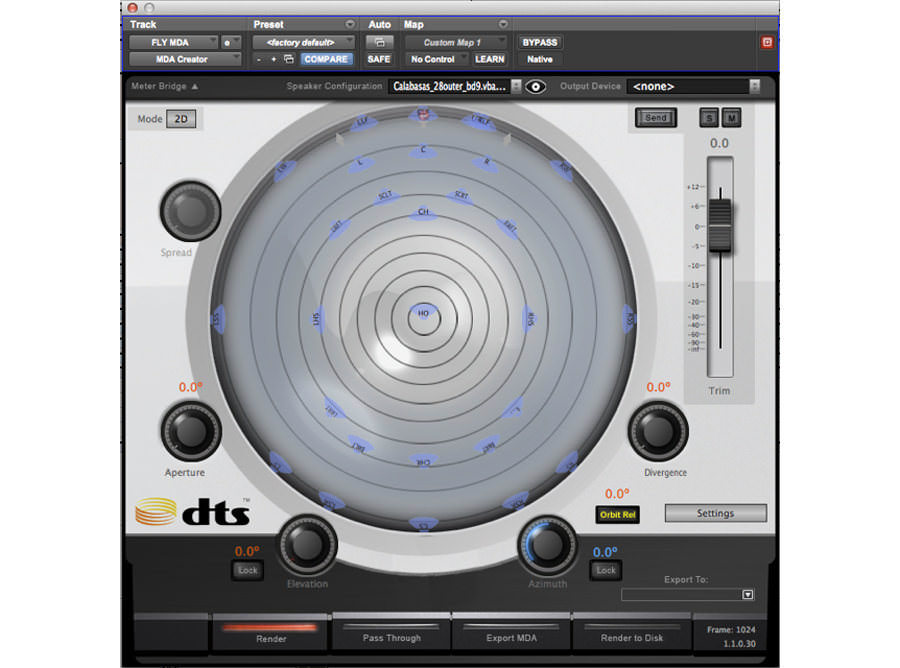
\includegraphics[scale=0.50]{figures/mdacreator.jpg}
	\caption {MDA Creator, DTS technology}
	\label{fig:mdacreator}
	\end{figure}

\chapter{Tecnica Vector Base Amplitude Panning VBAP}

In questo capitolo parleremo invece di cos'è la tecnica VBAP in modo da adattare l'MDA alle configurazioni di riproduzione 2.0, 5.1 e 4.0 .

Il \textbf{Vector Base Amplitude Panning VBAP} è una tecnica di spazializzazione audio che permette la localizzazione di  una sorgente sonora nello spazio attraverso la differenza di intensità di un dato segnale emesso tra due o più diffusori.

Immaginiamo di ascoltare una sorgente sonora posta da un lato di fronte a noi, lo stesso segnale sonoro emesso verrà captato da entrambe le nostre orecchie in modo diverso ed è proprio questa diversità che ci permette di capire la provenienza di un suono, infatti studi hanno definito la trasformazione che subisce il segnale sonoro captato da entrambe le orecchie in base all'angolo di provenienza del suono, questa trasformazione si chiama Head Related Transfer Function HRTF.

La HRTF pone le sue basi su tre fattori diversi:

\begin{itemize}
\item \textit{Interaural Intencity Difference IID} (si veda \cite{iid}) indica la differenza di intensità dello stesso segnale acustico che le nostre orecchie percepiscono in base all'angolo azimutale di provenienza del fronte sonoro.
\item \textit{Interaural Time  Difference ITD} indica il delay temporale che le nostre orecchie percepiscono in base all'angolo azimutale di provenienza.
\item \textit{frequency modification} indica come lo spettro in frequenza del segnale cambia anch'esso in base all'angolo di incidenza, a concorrere a questo fenomeno sta la presenza fisica della testa e del torso dell'ascoltatore (molta importanza ha la pinna dell'orecchio)
\end{itemize}

Per avere una ricostruzione sonora realistica (come avviene nell'ascolto binaurale) si dovrebbero usare tutti e tre questi fattori ma la tecnica VBAP prevede l'utilizzo solo della IID in quanto  prevede di riprodurre lo stesso segnale sonoro coerentemente\footnote{Con ''coerentemente'' intendo il fatto che il segnale deve essere emesso da tutti i diffusori nello stesso istante, non ci devono essere quindi slittamenti di fase} da un minimo di 2 diffusori ma con intensità differente.

Ora la cosa diventa abbastanza semplice in quanto se volgiamo ricreare una spazializzazione 2D basteranno un minimo di due diffusori, se invece vogliamo fare un 3D allora serviranno un minimo di 3 diffusori posti a triangolo, configurazioni del genere esistono già e sono state ampiamente testate ed affinate, per tutta la documentazione riguardante il VBAP si faccia riferimento a \cite{vbap}.

E' d'obbligo affrontare un po di matematica per riuscire poi ad adattare il VBAP alle configurazioni esposte in \ref{metodi}, partiamo subito con il caso bidimensionale con 2 diffusori affrontando la cosa direttamente con calcolo matriciale (all'inizio più difficile ma meglio generalizzabile per dopo).

\section{VBAP 2D}\label{c}

\begin{figure}[htbp]
	\centering
	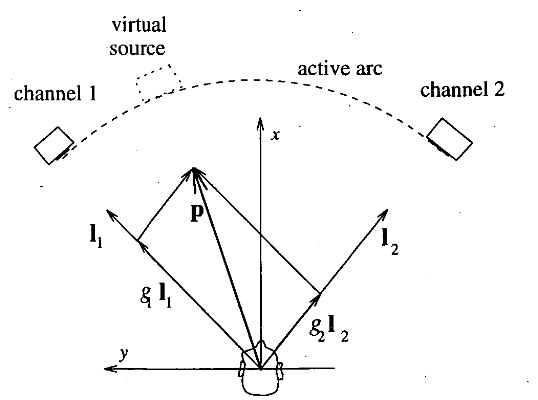
\includegraphics[scale=0.48]{figures/matrix2d.png}
	\caption {Composizione vettoriale delle sorgenti reali e virtuale}
	\label{fig:vettori2d}
	\end{figure}

Consideriamo un sistema cartesiano $ \boldsymbol{X},\boldsymbol{Y}$ in cui sono collocati due diffusori di cui conosciamo la posizione, definiamo come ''arco attivo'' la porzione di circonferenza compresa tra i due diffusori in cui vogliamo localizzare la sorgente virtuale, definisco poi $\boldsymbol{l_{1}}= {\left[ l_{11} \ l_{12} \right]}^T \ \  \boldsymbol{l_{2}}= {\left[ l_{21} \ l_{22} \right]}^T$ i vettori unitari che puntano verso i due altoparlanti e $\boldsymbol{p}= {\left[ p_1 \ p_2 \right]}^T$ il vettore unitario che punta verso la sorgente virtuale.

Come possiamo vedere dalla figura \ref{fig:vettori2d}, risulta semplicemente che $\boldsymbol{p}$ è combinazione lineare di $\boldsymbol{l_{1}}, \boldsymbol{l_{2}}$ con pesi rispettivamente 2 coefficienti che chiamerò $g_1$ e $g_2$, questi due valori non sono altro che i gain da applicare rispettivamente ai due diffusori per localizzare la sorgente virtuale nel punto indicato dal vettore $\boldsymbol{p}$.

Ora, conoscendo la posizione della nostra sorgente virtuale tramite $\boldsymbol{p}$, conoscendo i due vettori dei due diffusori $\boldsymbol{l_{1}}, \boldsymbol{l_{2}}$ le uniche incognite rimaste sono i 2 gain, ma è possibile trovare il loro valore in quanto è corretto definire la relazione: %definendo il vettore $\boldsymbol{g}= \left[ g_1 \ g_2 \right]$ posso scrivere la relazione:

\begin{equation}
\boldsymbol{p}= g_1 \boldsymbol{l_{1}} + g_2 \boldsymbol{l_{2}} %= \left[g_1 \ g_2 \right] \left[\boldsymbol{l_{1}} \ \boldsymbol{l_{2}} \right]^T 
\label{eq:bbbb}
\end{equation}

In questo caso però possiamo scompattare la scrittura in quanto:

\begin{equation}
\boldsymbol{p}=g_1 {\left[ l_{11} \ l_{12} \right]}^T + g_2 {\left[ l_{21} \ l_{22} \right]}^T= \left[ g_1 \ g_2 \right] \left[\begin{matrix}
l_{11} & l_{12}\\ l_{21} & l_{22}
\end{matrix} \right]
\label{eq:cccc}
\end{equation}

Ora trovando tutto in funzione dei due gain abbiamo che:

\begin{equation}
\left[g_1 \ g_2\right] = \left[ p_1 \ p_2 \right]  {\left[\begin{matrix}
l_{11} & l_{12}\\ l_{21} & l_{22}
\end{matrix} \right]}^{-1} \ \ \Rightarrow \ \ \ \boldsymbol{g}=\boldsymbol{p}^T {\boldsymbol{L_{12}}}^{-1}
\label{eq:dddd}
\end{equation}

Con $\boldsymbol{g}= \left[ g_1 \ g_2 \right]$ il vettore contenente i due gain e $\boldsymbol{L_{12}}$ la matrice $\left[\begin{matrix}
l_{11} & l_{12}\\ l_{21} & l_{22}
\end{matrix}\right]$ 

Logicamente assumo che la matrice $\boldsymbol{L_{12}}$ ammetta inversa\footnote{Per far si che la matrice ammetta inversa dovrà verificarsi che $\theta_0\neq 0°,90°$}, ora introducendo l'angolo $\theta_0$ e l'angolo $\theta$ come in figura \ref{fig:angoli} parametrizzo i vettori in funzione di essi nel modo seguente:

\[ p_1=cos(\theta),\ p_2=sen(\theta),\ l_{11}=cos(\theta_0),\ l_{12}=sen(\theta_0),\ l_{21}=cos(-\theta_0),\ l_{22}=sen(-\theta_0) \]

\begin{figure}[htbp]
	\centering
	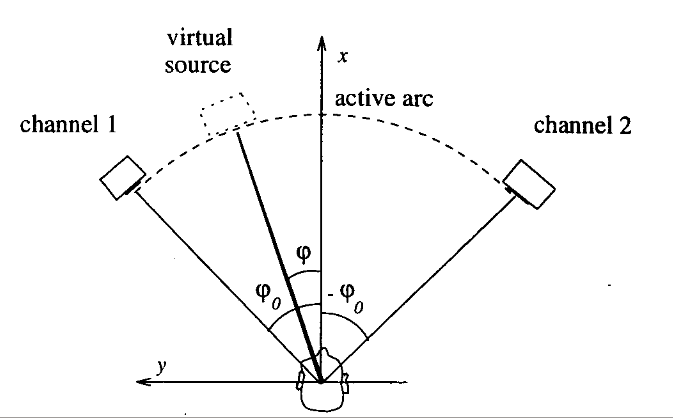
\includegraphics[scale=0.45]{figures/angoli.png}
	\caption {Angoli delle sorgenti reali e virtuale}
	\label{fig:angoli}
	\end{figure}

Fatto questo, essendo il nostro spazio ortogonale (cosa che giustifica la combinazione lineare scritta sopra), posso calcolare direttamente i coefficienti dei due gain invertendo prima la matrice e risolvendo la seguente equazione: 

\begin{equation}
\left[g_1 \ g_2\right] = \left[ cos(\theta) \ sen(\theta) \right]  {\left[\begin{matrix}
cos(\theta_0) & sen(\theta_0)\\ cos(-\theta_0) & sen(-\theta_0)
\end{matrix} \right]}^{-1} 
\label{eq:trigonometricmatrix}
\end{equation}

I due gain quindi risultano funzione dei due angoli in questo modo:

\begin{equation}\begin{split}
g_1=\dfrac{cos(\theta) sen(\theta_0) + sen (\theta) cos(\theta_0)}{2 cos(\theta_0) sen(\theta_0)}\\ \\
g_2=\dfrac{cos(\theta) sen(\theta_0) - sen (\theta) cos(\theta_0)}{2 cos(\theta_0) sen(\theta_0)}
\end{split}
\label{eq:eeee}
\end{equation}

Questi due coefficienti $g_1, g_2$ danno indicazioni su quanto segnale inviare a un diffusore rispetto all'altro ma non danno indicazioni su quale intensità sonora della sorgente virtuale percepiamo in quanto legata alle caratteristiche di diffusione, quindi introduciamo un coefficiente $C$ che indica il gain complessivo da applicare alla sorgente virtuale per ascoltare quest'ultimo con l'intensità sonora voluta, con l'accortezza però di riprodurre questo segnale con un solo diffusore posto sull'arco attivo, questo coefficiente andrà integrato in questo modo:

\begin{equation}
\left[g_1 \ g_2\right]_{scaled} = \dfrac{\sqrt{C} \left[ g_1 \ g_2 \right]}{\sqrt{g_1^2 + g_2^2}}
\label{eq:ffff}
\end{equation}

Spiegato il tutto nulla ci vieta poter estendere, con qualche accorgimento, questa tecnica ad $n$ diffusori, l'unica accortezza è che il nostro procedimento ne dovrà ''selezionare'' solo due per volta alla quale attribuire la realizzazione della sorgente virtuale, questa scelta si basa sulla posizione dei diffusori e dell'oggetto virtuale, infatti quest'ultimo potrà essere messo solo in un arco attivo per volta (l'intero arco giro è suddiviso in archi attivi che non si sovrappongono) quindi le due casse che delimitano questo arco saranno la coppia imputata a svolgere la riproduzione.

Consideriamo un numero $n$ arbitrario di casse consecutive $a_n$ disposte ad un angolo $\theta_{0,n}$ tali che $0°\leq \theta_{0,1},\ \theta_{0,2},\ \ldots,\ \theta_{0,n} <360°$, posizionando un qualsiasi oggetto virtuale in un qualsiasi angolo $\theta^{\prime}$ dovrà verificarsi che $\theta_{0,m}\leq \theta^{\prime} \leq \theta_{0,m+1}$ dove $m$ sta per il numero del diffusore adiacente alla sorgente virtuale ma con angolazione minore, quindi la coppia di casse da selezionare saranno $a_m$ e $a_{m+1}$, per rendere effettive le formule \ref{eq:eeee} ed \ref{eq:ffff} dovremo fare una piccola modifica in quanto dovremo assumere:

\begin{equation}
\theta_0 = \dfrac{\theta_{0,m+1}-\theta_{0,m}}{2} \ \ \ \ \ \theta=\theta^{\prime}-\dfrac{\theta_{0,m+1}+\theta_{0,m}}{2}
\label{phidiverso}
\end{equation}

Detto questo $g_{1,scaled}$ e $g_{2,scaled}$ non saranno altro che i gain da applicare rispettivamente alla coppia di diffusori $a_{m} , a_{m+1}$.
 \begin{figure}[htbp]
	\centering
	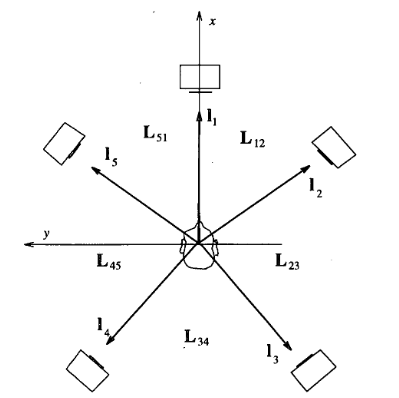
\includegraphics[scale=0.55]{figures/matrix5-1.png}
	\caption {VBAP bidimensionale con più altoparlanti}
	\label{fig:angoli5}
	\end{figure}



\section{VBAP 3D}

Capito qual'è il modello e l'algoritmo di implementazione del VBAP in due dimensioni ne estenderemo il concetto a tre (non mi soffermerò troppo su questa estensione in quanto non servirà ai fini della continuazione della tesi).

Il modo più semplice per realizzare questa tecnica in 3D è disporre tre diffusori ai vertici di un triangolo equilatero come in figura \ref{fig:triangolo} e per analogia prendere i procedimenti e le formule esposte nel paragrafo \ref{c} integrandole la dimensione $\boldsymbol{Z}$, per fare questo introduciamo l'angolo $\phi$ che indica l'elevazione dal piano orizzontale.

\begin{figure}[htbp]
	\centering
	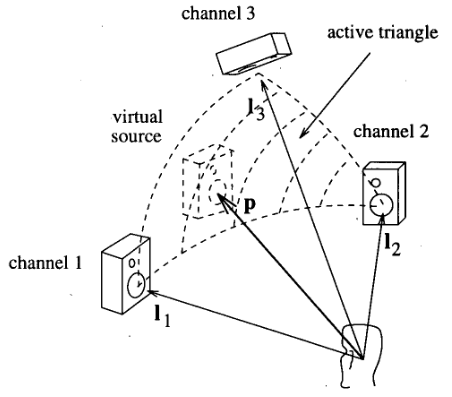
\includegraphics[scale=0.50]{figures/matrix3d.png}
	\caption {Composizione vettoriale delle sorgenti reali e virtuale in tre dimensioni}
	\label{fig:triangolo}
	\end{figure}

Cominciamo non considerando più il concetto di arco attivo ma penseremo invece che che la sorgente virtuale potrà essere collocata nella calotta\footnote{Con calotta si intende una porzione di superficie di una sfera.} attiva delimitata dalle rette congiungenti gli altoparlanti a due a due,	 quindi esattamente come sopra se definiamo i vettori unitari che puntano alle tre casse come $ \boldsymbol{l_{1}}= {\left[ l_{11} \ l_{12} \ l_{13} \right]}^T \ \ \boldsymbol{l_{2}}= {\left[ l_{21} \ l_{22} \ l_{23} \right]}^T \ \ \boldsymbol{l_{3}}= {\left[ l_{31} \ l_{32} \ l_{33} \right]}^T$ e il vettore della sorgente virtuale $\boldsymbol{p}= {\left[ p_{1} \ p_{2} \ p_{3} \right]}^T$ risulta che:

\begin{equation}
\boldsymbol{p} = \left[ g_1 \ g_2 \ g_3 \right] \left[ \boldsymbol{l_{1}} \ \boldsymbol{l_{2}} \ \boldsymbol{l_{3}} \right]^T
\label{gggg}
\end{equation}

Quindi ribaltando l'equazione ci rimane che:

\begin{equation}
\left[g_1 \ g_2 \ g_3 \right] = \left[ p_1 \ p_2 \ p_3 \right]  {\left[\begin{matrix}
l_{11} & l_{12} & l_{13}\\ l_{21} & l_{22} & l_{23} \\ l_{31} & l_{32} & l_{33}
\end{matrix} \right]}^{-1} \ \ \Rightarrow \ \ \ \boldsymbol{g}=\boldsymbol{p}^T {\boldsymbol{L_{123}}}^{-1}
\label{hhhh}
\end{equation}

Anche in questo caso possiamo calcolare i tre coefficienti scalati, analogamente a sopra, in questa maniera:

\begin{equation}
\left[g_1 \ g_2 \ g_3 \right]_{scaled} = \dfrac{\sqrt{C} \left[ g_1 \ g_2 \ g_3 \right]}{\sqrt{g_1^2 + g_2^2 + g_3^2}}
\label{iiii}
\end{equation}

In questo caso fare un esempio non è possibile in quanto il VBAP in tre dimensioni è molto legato alla geometria di implementazione e la trigonometria sulla sfera è analiticamente pesante anche se possibile, quindi si preferisce lasciare al calcolatore il compito del calcolo vettoriale senza lasciare a noi il compito di tradurre il tutto in funzioni angolari, si veda per esempio il passaggio dalla formula \ref{eq:dddd} alla formula \ref{eq:eeee}. 

Ora, come sopra, possiamo arrivare ad un numero $n$ di altoparlanti per coprire tutto l'angolo solido, anche qui il nostro algoritmo dovrà ''selezionare'' gli altoparlanti che saranno imputati alla riproduzione del nostro oggetto sonoro, gli stessi che delimiteranno la calotta attiva che racchiude la sorgente virtuale.

\begin{figure}[htbp]
	\centering
	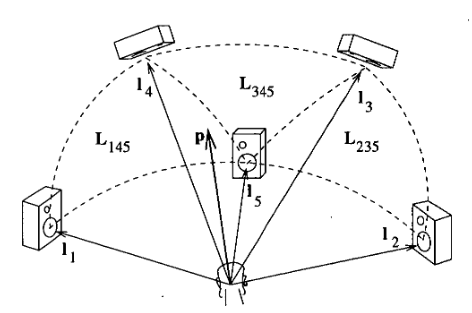
\includegraphics[scale=0.50 ]{figures/matrix3dfull.png}
	\caption {Configurazione a più altoparlanti per la tecnica VBAP in tre dimensioni}
	\label{fig:matrix3dfull}
	\end{figure}


\chapter{Adattamento del formato MDA con la tecnica VBAP}

Ricapitolando siamo arrivati al punto di sapere cos'è il formato MDA e che cos'è la tecnica di spazializzazione VBAP,
il passo successivo è riuscire ad integrare il formato MDA alle configurazioni 2.0, 5.1 e 4.0 con la tecnica sopra proposta.

Un concetto fondamentale da ricordare è che dentro il formato a oggetti MDA i metadati danno informazioni principalmente sulla posizione e sull'estensione dell'oggetto, in questo caso però lo studio introduttivo del VBAP fatto nel capitolo precedente non tiene conto dei parametri di estensione quali la divergence, la aperture e la coherence, quindi nell'adattamento ai formati proposti considererò solo il posizionamento spaziale di una sorgente monofonica.

Ricordiamoci anche che le informazioni riguardanti la posizione relative agli oggetti sonori fanno riferimento ad uno spazio tridimensionale, quindi esse si adatteranno benissimo a una riproduzione VBAP tridimensionale, se però il tipo di riproduzione è svolto in un piano come nel nostro caso, allora bisognerà adattare le informazioni contenute nei metadati in modo da poter essere congruenti all configurazione che andranno a pilotare, logicamente queste trasformazioni dovranno il più possibile lasciare inalterata la percezione spaziale a quella che è stato decisa in fase di post-produzione.

Anche qui salta all'occhio la potenza dell'audio ad oggetti, nell'audio channel-oriented per adattare un tipo di riproduzione ad un altro dovevamo attuare trasformazioni direttamente ai segnali contenenti le informazioni sonore, nell'audio object-oriented invece dobbiamo solo fare delle trasformazioni delle coordinate degli oggetti sonori.

\section{Adattamento MDA in configurazioni tridimensionali, planari e lineare}

Per quanto riguarda l'adattamento alle geometrie tridimensionali non c'è bisogno di fare delle trasformazioni sulle coordinate in quante esse possono essere applicate direttamente, l'unica cosa che c'è da fare è un piccolo discorso sulle distanze e sui raggi.

Introduciamo due raggi: $r_0$ che sarebbe la lunghezza del vettore congiungente l'ascoltatore con uno degli diffusori (non importa quale dato che tutti gli diffusori sono posizionati sulla superficie di una sfera quindi si avranno tutti raggi uguali) e definiamo $r_1$ come la lunghezza del vettore congiungente l'ascoltatore e il più vicino degli oggetti virtuali che si vuole riprodurre, premettendo che con la tecnica VBAP posso solo creare sorgenti virtuali a partire dalla superficie della sfera verso l'esterno, allora qualsiasi di questi che avranno $r_n < r_0$ non sarò in grado di riprodurli nella maniera corretta, quindi dovrò attuare una trasformazione in modo da lasciare inalterata la distanza relativa fra le sorgenti virtuali in questo modo:

\begin{equation}
\left\{\begin{matrix}
se\ \  r_1 < r_0\ \ \Rightarrow \ \ r_n^{\prime} = r_n+(r_0 - r_1) \\
\\
se\ \  r_1 \geq r_0\ \ \Rightarrow \ \ r_n^{\prime} = r_n\\
\end{matrix}\right.
\label{jjjj}
\end{equation}

Così facendo traslo la posizione virtuale di tutti gli oggetti al di fuori (o al massimo nella) sfera creata sommando le calotte attive.

Fatte le trasformazioni sui raggi, non ci rimane che introdurre degli aspetti che ci giustifichino la sensazione di lontananza dell'oggetto; questi aspetti sono l'intensità sonora, l'attenuazione delle alte frequenze, il rapporto riverbero/segnale diretto e il delay temporale. 

Volendo partire dall'intensità sonora riprendiamo ciò che è stato detto nel paragrafo \ref{c}: il fattore $C$ è legato al gain complessivo dell'oggetto ma quest'ultimo posizionato sulla superficie della sfera, ora sappiamo dalla formula \ref{jjjj} che ogni oggetto è posizionato o sulla sfera o al suo esterno quindi possiamo prenderci la libertà di moltiplicare $C$ per un coefficiente $f^{\prime}$ che ne scali il contenuto in base alla distanza dell'oggetto, in questo modo:

\begin{equation}
\boldsymbol{g_{n\ scaled}} = \dfrac{\sqrt{C_n \ f^{\prime}}\ \boldsymbol{g_n}}{\sqrt{g_1^2 +g_2^2 + g_3^2}} \ \ \ con \ \ \ \left\{\begin{matrix}
f^{\prime}= \frac{arctan\left((r_n^{\prime}-r_0)\ \dfrac{\pi}{2}\right)}{(r_n^{\prime}-r_0)\ \dfrac{\pi}{2}} & per\ r_n^{\prime}>r_0
\\
f^{\prime}=1 & per\ r_n^{\prime}=r_0
\end{matrix}\right.
\label{kkkk}
\end{equation}

In teoria l'ampiezza di un segnale sonoro dovrebbe calare con l'inverso della distanza e quindi nel nostro caso come $f=\frac{1}{r_n^{\prime}-r_0}$ ma facendo così avremmo dei problemi di divergenza per $r_n^{\prime}=r_0$ e valori sovrastimati per la differenza $r_n^{\prime}-r_0<1$, quindi in accordo con quanto scritto in \cite{distanza} introduco la funzione $f^{\prime}$ che approssima il più possibile la funzione originale ma che risolve totalmente i problemi nelle zone difficili (figura \ref{fig:distance}).

\begin{figure}[htbp]
	\centering
	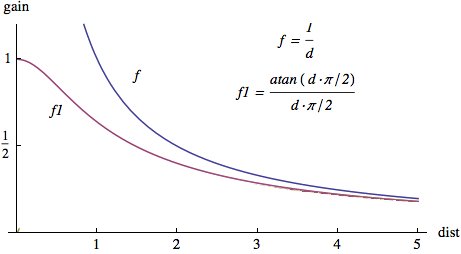
\includegraphics[scale=0.60]{figures/distance.png}
	\caption {Funzione distanza originale e funzione approssimata}
	\label{fig:distance}
	\end{figure}

Logicamente quanto detto qui sopra dovrà essere applicato in tutti casi di VBAP sia tridimensionale che non.

Per quanto riguarda le informazioni relative agli ultimi tre aspetti descritti sopra, possiamo dire che si possono optare due strade: la prima è di inserirli direttamente negli oggetti sonori nella fase di produzione operando delle trasformazioni del segnale e memorizzando nel formato gli oggetti già modificati\footnote{In realtà in questa maniera ogni operazione sui raggi si ripercuoterebbe negativamente su questi tre fattori introducendo un'errore ma che possiamo considerare trascurabile visto l'entità ridotta delle trasformazioni data dalla ridotta dimensione spaziale di un impianto casalingo.} oppure una seconda strada può essere di lasciare direttamente al DSP dell'impianto il compito di operare le trasformazioni sui sugli oggetti sonori lasciati precedentemente inalterati dal produttore.

Se si seguisse quest'ultima via, il DSP dovrebbe avere al suo interno alcuni algoritmi che si occupino del riverbero e del filtraggio delle alte frequenze entrambi in funzione del parametro spaziale $r_n^{\prime}-r_0$  \footnote{Non indico semplicemente il parametro spaziale $r_n^{\prime}$ in quanto già il comportamento acustico che si verifica tra l'ascoltatore e la distanza $r_0$ concorre al verificarsi di questi effetti} e che si occupi del delay temporale   con un $\tau$ dato dalla formula \ref{eq:tau}, con $c$ velocità del suono in aria.

\begin{equation}
\tau_{n} = \dfrac{r_n^{\prime}-r_0}{c}
\label{eq:tau}
\end{equation}



Introduciamo ora la riproduzione di un programma sonoro tridimensionale in un impianto planare.  questo aspetto va preso con i guanti in quanto la riproduzione o meno tramite il VBAP in due dimensioni dipende dalla posizione dell'oggetto, mi spiego meglio:

Nei metadati del formato MDA sono presenti gli angoli $\theta, \phi$ e il raggio $r$ che identificano la posizione sul piano di ascolto bidimensionale, quello che ci da informazioni sull'altezza è l'angolo (appunto detto di elevazione) $\phi$, ponendo semplicemente $\phi=0°$ elimineremmo la dimensione verticale ma comprometteremmo anche la percezione degli oggetti originariamente posti sopra l'ascoltatore.

Per esempio, mettiamo il caso che un oggetto sia posto ad un angolo $	\theta= 90° $ e un angolo $\phi=89°$, esso praticamente si trova quasi perfettamente al disopra della nostra testa, a primo acchito verrebbe da pensare di porre semplicemente quest'ultimo a $0°$ ma si avrebbe uno spostamento netto dell'oggetto alla completa sinistra dell'ascoltatore il che è incongruente con la scelta iniziale del produttore, quindi si capisce che questa strada è concettualmente sbagliata.

Contrariamente un oggetto posto, per esempio, a $\theta= 90°$ con un angolo $\phi=45°$ e $r$ abbastanza grande comparato con il raggio $r_0$, posso tranquillamente pensarlo come proveniente solamente da sinistra visto la sua distanza dall'ascoltatore, quindi riproducibile con un VBAP in due dimensioni.

Vediamo ora come faccio a selezionare gli oggetti non posti su piano orizzontale adatti alla riproduzione con la tecnica VBAP 2D: per prima cosa sposto tutti gli oggetti della semisfera inferiore sopra l'ascoltatore in questo modo:

\begin{equation}
\phi_{n,top} = arctg  \left( \dfrac{\vert sen(\phi_n) \vert}{ cos(\phi_n) } \right)
\label{  b}
\end{equation}

Successivamente, tracciando la proiettante dell'oggetto nel piano orizzontale, si può vedere che quelli che soddisfano l'equazione \ref{zzz} possono essere riprodotti con il VBAP tralasciando l'angolo azimutale e considerando le formule del capitolo \ref{c}.

\begin{equation}
r_{n,shadow}=r_n^{\prime} cos(\phi_{n,top}) \geq r_0
\label{zzz}
\end{equation}

Tutti gli altri oggetti invece no, ma una soluzione a questi ultimi potrebbe essere di creare un ascolto immersivo per questi sfruttando tutti i diffusori del piano di ascolto e scalando il segnale da inviare a tutti questi ultimi in base alla posizione della proiettante dell'oggetto sul piano, per esempio, nel primo caso sopra, la proiettante dell'oggetto sarebbe un punto molto vicino all'ascoltatore immediatamente alla sua sinistra, quindi i due diffusori a sinistra dovrebbero riprodurre con la metà più un poco di intensità il segnale attribuito all'oggetto, invece gli diffusori a destra dovrebbero riprodurre il segnale con la differenza di intensità per arrivare al totale.

Un oggetto invece posto esattamente sopra l'ascoltatore potrebbe essere ricreato inviando un segnale a tutti gli $n$ diffusori scalato come $\frac{1}{\sqrt{n}}$.

Sicuramente in letteratura una tecnica che risolva la situazione appena citata esiste già, ma non essendo inerente alla spiegazione della tecnica VBAP non verrà discussa in questo testo.


Per ultimo vediamo come adattare il formato alla configurazione monodimensionale, ho parlato al singolare in quanto a meno di configurazioni esoteriche si utilizzerà sempre il sistema con due diffusori posti di fronte all'ascoltatore\footnote{Al contrario del surround in cui è più facile trovare diverse configurazioni}, bisogna qui stravolgere il formato in maniera pesante in quanto si devono sottrarre ben due dimensioni ma paradossalmente i passaggi da fare sono più semplici.

Come prima cosa dovrò spostare tutti gli oggetti che originariamente sono posti dietro (quindi con angoli compresi tra $90°$ e $270°$) davanti all'ascoltatore operando una trasformazione sull'angolo azimutale:

\begin{equation}
\theta_{n,front} = arctg  \left( \dfrac{sen(\theta_n)}{\vert cos(\theta_n)\vert } \right)
\label{llll}
\end{equation}

In questo modo tutti gli angoli azimutali di ogni oggetto saranno posti tra $-90° \leq \theta_{n,front} \leq +90°$.

Abbiamo così ottenuto oggetti posti al massimo perfettamente ai nostri fianchi ma le configurazioni planari prevedono al massimo una riproduzione di oggetti a $\pm \theta_0$ data dalla limitata ampiezza angolare dei diffusori, quindi dovrò rimappare gli angoli appena ottenuti in modo da essere compresi tra $0°\ e \pm \theta_0$.

Come primo approccio ho pensato semplicemente di dividere per un fattore tre gli angoli ma accade che gli oggetti posti sullo scenario frontale vengono schiacciati troppo verso l'origine, quindi ho optato per la funzione seno (usata come peso) che schiacciasse gli oggetti posti sui lati e che lasciasse il più inalterati possibile gli angoli degli oggetti posti di fronte, in più il tutto viene ulteriormente scalato per il coseno dell'angolo di elevazione per tenere conto di quest'ultimo e della proiezione del vettore sul piano orizzontale, in questo modo:

\begin{equation}
\theta_{n, remapped}= \theta_0 \cos(\phi) \ sen (\theta_{n,front}) = \theta_0 \cos(\phi)\ sen \left( arctg  \left( \dfrac{sen(\theta_n)}{\vert cos(\theta_n)\vert } \right)\right)
\label{mmmm}
\end{equation}

\section{Esempio di integrazione con sistemi 4.0, 5.1 e 2.0}

Ora praticamente l'adattamento è fatto, nel capitolo precedente si è visto come rimappare le coordinate degli oggetti in modo scalare da una configurazione tridimensionale a una planare e lineare, poi conoscendo come si usa la tecnica VBAP posso tranquillamente riprodurre nelle configurazioni 2.0, 5.1 e 4.0, rimane ora solo da impostare di volta in volta gli angoli $\theta_{0,n}$ nelle configurazioni considerate ed applicare il tipo di VBAP adatto (bi o tridimensionale).

Consideriamo un file .mda in cui siano inseriti tre oggetti sonori statici con annessi metadati contenenti le seguenti coordinate sferiche:\\

\begin{tabular}{|c|c|c|c|c|}
\hline
oggetto 1 & $\theta_1=15°$ & $\phi_1=0°$ & $r_1=1,5m$ & $C_1=1,3$ \\
\hline
oggetto 2 & $\theta_2=275°$ & $\phi_2=0°$ & $r_2=2,5m$ & $C_2=1,6$ \\
\hline
oggetto 3 & $\theta_3=160°$ & $\phi_3=45°$ & $r_3=3,0m$ & $C_1=0,8$ \\
\hline

\end{tabular} \\ \\

N.B) ai fini dei calcoli conviene pensare $\theta_2=275°$ come $\theta_2=-85°$.\\

Conoscendo questi valori abbiamo tutto per poter riprodurre l'oggetto in una configurazione voluto attraverso il VBAP, da notare è che ho fatto un esempio di tre oggetti che rimangono fissi nel tempo ma se volessi farli muovere basterebbe ripetere il procedimento esposto ad ogni istante con le coordinate riferite a quel particolare lasso temporale.

Cominciamo con la configurazione 4.0, una possibile disposizione di diffusori potrebbe essere questa:\\

\begin{tabular}{|c|c|c|}
\hline
diffusore 1 & $\theta_{0,1}=45°$ & $r_0=2m$\\
\hline
diffusore 2 & $\theta_{0,2}=135°$ & $r_0=2m$\\
\hline
diffusore 3 & $\theta_{0,3}=-135°$ & $r_0=2m$\\
\hline
diffusore 4 & $\theta_{0,4}=-45°$ & $r_0=2m$\\
\hline
\end{tabular} \\
\\

Come prima cosa applichiamo la formula \ref{jjjj} in modo da scalare i raggi degli oggetti e rendergli:

\[r_1^{\prime}=2m \ \  r_2^{\prime}=3m \ \ r_3^{\prime}=3,5m  \]

Ora è facile trovare i gain e i gain scalati del primo e del secondo oggetto in quanto il primo è riprodotto dai diffusori 4 e 1 invece il secondo dai diffusori 3 e 4 con questo procedimento:

per entrambi gli oggetti, prima applico la formula \ref{phidiverso} in modo da trovare i nuovi angoli da mettere nella formula \ref{eq:eeee}, poi considerando i coefficienti $C_n$ e i raggi $r_n^{\prime}$ ricavo dalla formula \ref{kkkk} i gain scalati per entrambi gli oggetti che in questo caso saranno:

\begin{equation}
\begin{matrix}
g_{(1,obj\ 1)} = 0,87 & g_{(1,obj\ 1)scaled} = 0,861\\
g_{(4,obj\ 1)} = 0,50 & g_{(4,obj\ 1)scaled} = 0,733\\
g_{(4,obj\ 2)} = 0,76 & g_{(4,obj\ 2)scaled} = 0,779\\
g_{(3,obj\ 2)} = 0,64 & g_{(3,obj\ 2)scaled} = 0,651\\
\end{matrix}
\label{gscalatiesempio1}
\end{equation}
\\

Passiamo ora all'adattamento alla configurazione 5.1.

Una possibile configurazione di impianto 5.1 potrebbe essere la seguente:

\begin{tabular}{|c|c|c|}
\hline
diffusore 1 & $\theta_{0,1}=0°$ & $r_0=2m$\\
\hline
diffusore 2 & $\theta_{0,2}=30°$ & $r_0=2m$\\
\hline
diffusore 3 & $\theta_{0,3}=110°$ & $r_0=2m$\\
\hline
diffusore 4 & $\theta_{0,4}=-110°$ & $r_0=2m$\\
\hline
diffusore 5 & $\theta_{0,4}=-30°$ & $r_0=2m$\\
\hline
\end{tabular} \\
\\

Non ci rimane che operare nella stessa maniera utilizzata per la configurazione 4.0 esposta appena sopra (infatti si applicheranno esattamente le stesse formule con l'unica differenza di avere dei $\theta_{0,n}$ visibilmente diversi), ricavo così i gain e i gain scalati degli diffusori 2 e 1 (imputati alla riproduzione del primo oggetto) e 5 e 4 (imputati alla riproduzione del secondo):

\begin{equation}
\begin{matrix}
g_{(2,obj\ 1)} = 0,52 & g_{(2,obj\ 1)scaled} = 0,806\\
g_{(1,obj\ 1)} = 0,52 & g_{(1,obj\ 1)scaled} = 0,806\\
g_{(5,obj\ 2)} = 0,43 & g_{(5,obj\ 2)scaled} = 0,465\\
g_{(4,obj\ 2)} = 0,83 & g_{(4,obj\ 2)scaled} = 0,898  \\

\end{matrix}
\label{gscalatiesempio2}
\end{equation} \\


Volutamente, per entrambe le configurazioni, ho tralasciato la riproduzione del terzo oggetto in modo da riprenderlo qui, infatti per prima cosa bisogna vedere se esso verifica l'equazione \ref{zzz} cosa che avviene, poi si provvede a calcolare normalmente i gain e i gain scalati della oggetto rispettivamente nelle configurazioni 4.0 e 5.1 dando i seguenti risultati:

\begin{equation}
\begin{matrix}
g_{(3,obj\ 3)} = 0,42 & g_{(3,obj\ 3)scaled} = 0,266\\
g_{(2,obj\ 3)} = 0,90 & g_{(2,obj\ 3)scaled} = 0,571\\
\\
g_{(4,obj\ 3)} = 1,19 & g_{(4,obj\ 3)scaled} = 0,383\\
g_{(3,obj\ 3)} = 1,55 & g_{(3,obj\ 3)scaled} = 0,499\\

\end{matrix}
\label{gscalatiesempiooggetto3}
\end{equation} \\



Per ultimo esempio vediamo il risultato dell'adattamento alla configurazione 2.0.

Una configurazione possibile potrebbe essere la seguente:
\\

\begin{tabular}{|c|c|c|}
\hline
diffusore 1 & $\theta_{0,1}=30°$ & $r_0=2m$\\
\hline
diffusore 2 & $\theta_{0,2}=-30°$ & $r_0=2m$\\
\hline
\end{tabular} \\
\\

Applicando rispettivamente la formula \ref{llll} e la formula \ref{mmmm} ottengo i seguenti risultati:


\begin{tabular}{|c|c|}
\hline
$\theta_{1,front} = 15°$     & $\theta_{1,remapped} =  8°  $   \\
\hline
$\theta_{2,front} = -85°$     & $\theta_{2,remapped} = -29° $     \\
\hline
$\theta_{3,front} = 20°$    & $ \theta_{3,remapped} =  7° $    \\
\hline
\end{tabular} \\
\\

Ora non ci rimane che trovare i gain degli oggetti tramite la formula \ref{eq:eeee} e i gain scalati con la \ref{kkkk}.

\begin{equation}
\begin{matrix}
g_{(1,obj\ 1)} = 0,71 & g_{(1,obj\ 1)scaled} = 0,975\\
g_{(2,obj\ 1)} = 0,43 & g_{(2,obj\ 1)scaled} = 0,590\\
g_{(1,obj\ 2)} = 0,02 & g_{(1,obj\ 2)scaled} = 0,021\\
g_{(2,obj\ 2)} = 0,99 & g_{(2,obj\ 2)scaled} = 1,011\\
g_{(1,obj\ 3)} = 0,69 & g_{(1,obj\ 3)scaled} = 0,524\\
g_{(2,obj\ 3)} = 0,46 & g_{(2,obj\ 3)scaled} = 0,349\\
\end{matrix}
\label{gscalatiesempio3}
\end{equation}










\chapter*{Conclusioni}

Sviluppando questa tesi quindi, è stata affrontata la filosofia di implementazione dell'audio a oggetti e si è visto la sua utilità e versatilità nel campo del audio-video e del solo audio implementandola nelle configurazioni di riproduzione 2.0, 4.0 e 5.1 attraverso la tecnica di spazializzazione VBAP.

Questo sviluppo però getta solo le basi del suo impiego, si dovrà approfondire di più l'argomento per raffinarlo e renderlo fruibile.




\addcontentsline{toc}{chapter}{Conclusioni}

\begin{thebibliography}{}

\bibitem{5.1} \textit{https://www.itu.int/dms\_pubrec/itu-r/rec/bs/R-REC-BS.775-3-201208-I!!PDF-E.pdf}
\bibitem{digital} \textit{https://it.wikipedia.org/wiki/Dolby\_Digital}
\bibitem{surround} \textit{http://www.dith.it/listing/master/dispense\%20Schiavoni/CSE10-08.pdf}
\bibitem{object} \textit{http://archive.afsi.eu/download/sites/default/files/uploads/mda\_white\_paper.pdf}
\bibitem{atmos} \textit{https://www.dolby.com/us/en/technologies/dolby-atmos/dolby-atmos-next-generation-audio-for-cinema-white-paper.pdf}
\bibitem{mda}\textit{http://www.etsi.org/deliver/etsi\_ts/103200\_103299/103223/01.01.01\_60/ts\_103223v010101p.pdf}
\bibitem{uri} \textit{https://www.rfc-editor.org/rfc/pdfrfc/rfc3986.txt.pdf}
\bibitem{creator}\textit{//digitalcommons.calpoly.edu/cgi/viewcontent.cgi?article=1049}\&\textit{context=laessp}
\bibitem{iid} \textit{https://en.wikipedia.org/wiki/Sound\_localization\#ITD\_and\_IID}
\bibitem{vbap} \textit{http://lib.tkk.fi/Diss/2001/isbn9512255324/article1.pdf}
\bibitem{distanza} \textit{http://write.flossmanuals.net/csound/b-panning-and-spatialization/}
\end{thebibliography}

\addcontentsline{toc} {chapter}{Bibliografia}


\end{document}
